\documentclass[journal,12pt,twocolumn]{IEEEtran}
%
\usepackage{setspace}
\usepackage{gensymb}
%\doublespacing
\singlespacing

%\usepackage{graphicx}
%\usepackage{amssymb}
%\usepackage{relsize}
\usepackage[cmex10]{amsmath}
%\usepackage{amsthm}
%\interdisplaylinepenalty=2500
%\savesymbol{iint}
%\usepackage{txfonts}
%\restoresymbol{TXF}{iint}
%\usepackage{wasysym}
\usepackage{amsthm}
%\usepackage{iithtlc}
\usepackage{mathrsfs}
\usepackage{txfonts}
\usepackage{stfloats}
\usepackage{bm}
\usepackage{cite}
\usepackage{cases}
\usepackage{subfig}
%\usepackage{xtab}
\usepackage{longtable}
\usepackage{multirow}
%\usepackage{algorithm}
%\usepackage{algpseudocode}
\usepackage{enumitem}
\usepackage{mathtools}
\usepackage{steinmetz}
\usepackage{tikz}
\usepackage{circuitikz}
\usepackage{verbatim}
\usepackage{tfrupee}
\usepackage[breaklinks=true]{hyperref}
%\usepackage{stmaryrd}
\usepackage{tkz-euclide} % loads  TikZ and tkz-base
%\usetkzobj{all}
\usetikzlibrary{calc,math}
\usepackage{listings}
    \usepackage{color}                                            %%
    \usepackage{array}                                            %%
    \usepackage{longtable}                                        %%
    \usepackage{calc}                                             %%
    \usepackage{multirow}                                         %%
    \usepackage{hhline}                                           %%
    \usepackage{ifthen}                                           %%
  %optionally (for landscape tables embedded in another document): %%
    \usepackage{lscape}     
\usepackage{multicol}
\usepackage{chngcntr}
%\usepackage{enumerate}

%\usepackage{wasysym}
%\newcounter{MYtempeqncnt}
\DeclareMathOperator*{\Res}{Res}
%\renewcommand{\baselinestretch}{2}
\renewcommand\thesection{\arabic{section}}
\renewcommand\thesubsection{\thesection.\arabic{subsection}}
\renewcommand\thesubsubsection{\thesubsection.\arabic{subsubsection}}

\renewcommand\thesectiondis{\arabic{section}}
\renewcommand\thesubsectiondis{\thesectiondis.\arabic{subsection}}
\renewcommand\thesubsubsectiondis{\thesubsectiondis.\arabic{subsubsection}}

% correct bad hyphenation here
\hyphenation{op-tical net-works semi-conduc-tor}
\def\inputGnumericTable{}                                 %%

\lstset{
%language=C,
frame=single, 
breaklines=true,
columns=fullflexible
}
%\lstset{
%language=tex,
%frame=single, 
%breaklines=true
%}

\begin{document}
%


\newtheorem{theorem}{Theorem}[section]
\newtheorem{problem}{Problem}
\newtheorem{proposition}{Proposition}[section]
\newtheorem{lemma}{Lemma}[section]
\newtheorem{corollary}[theorem]{Corollary}
\newtheorem{example}{Example}[section]
\newtheorem{definition}[problem]{Definition}
%\newtheorem{thm}{Theorem}[section] 
%\newtheorem{defn}[thm]{Definition}
%\newtheorem{algorithm}{Algorithm}[section]
%\newtheorem{cor}{Corollary}
\newcommand{\BEQA}{\begin{eqnarray}}
\newcommand{\EEQA}{\end{eqnarray}}
\newcommand{\define}{\stackrel{\triangle}{=}}

\bibliographystyle{IEEEtran}
%\bibliographystyle{ieeetr}


\providecommand{\mbf}{\mathbf}
\providecommand{\pr}[1]{\ensuremath{\Pr\left(#1\right)}}
\providecommand{\qfunc}[1]{\ensuremath{Q\left(#1\right)}}
\providecommand{\sbrak}[1]{\ensuremath{{}\left[#1\right]}}
\providecommand{\lsbrak}[1]{\ensuremath{{}\left[#1\right.}}
\providecommand{\rsbrak}[1]{\ensuremath{{}\left.#1\right]}}
\providecommand{\brak}[1]{\ensuremath{\left(#1\right)}}
\providecommand{\lbrak}[1]{\ensuremath{\left(#1\right.}}
\providecommand{\rbrak}[1]{\ensuremath{\left.#1\right)}}
\providecommand{\cbrak}[1]{\ensuremath{\left\{#1\right\}}}
\providecommand{\lcbrak}[1]{\ensuremath{\left\{#1\right.}}
\providecommand{\rcbrak}[1]{\ensuremath{\left.#1\right\}}}
\theoremstyle{remark}
\newtheorem{rem}{Remark}
\newcommand{\sgn}{\mathop{\mathrm{sgn}}}
\providecommand{\abs}[1]{\left\vert#1\right\vert}
\providecommand{\res}[1]{\Res\displaylimits_{#1}} 
\providecommand{\norm}[1]{\left\lVert#1\right\rVert}
%\providecommand{\norm}[1]{\lVert#1\rVert}
\providecommand{\mtx}[1]{\mathbf{#1}}
\providecommand{\mean}[1]{E\left[ #1 \right]}
\providecommand{\fourier}{\overset{\mathcal{F}}{ \rightleftharpoons}}
%\providecommand{\hilbert}{\overset{\mathcal{H}}{ \rightleftharpoons}}
\providecommand{\system}{\overset{\mathcal{H}}{ \longleftrightarrow}}
	%\newcommand{\solution}[2]{\textbf{Solution:}{#1}}
\newcommand{\solution}{\noindent \textbf{Solution: }}
\newcommand{\cosec}{\,\text{cosec}\,}
\providecommand{\dec}[2]{\ensuremath{\overset{#1}{\underset{#2}{\gtrless}}}}
\newcommand{\myvec}[1]{\ensuremath{\begin{pmatrix}#1\end{pmatrix}}}
\newcommand{\mydet}[1]{\ensuremath{\begin{vmatrix}#1\end{vmatrix}}}
%\numberwithin{equation}{section}
\numberwithin{equation}{subsection}
%\numberwithin{problem}{section}
%\numberwithin{definition}{section}
\makeatletter
\@addtoreset{figure}{problem}
\makeatother

\let\StandardTheFigure\thefigure
\let\vec\mathbf
%\renewcommand{\thefigure}{\theproblem.\arabic{figure}}
\renewcommand{\thefigure}{\theproblem}
%\setlist[enumerate,1]{before=\renewcommand\theequation{\theenumi.\arabic{equation}}
%\counterwithin{equation}{enumi}


%\renewcommand{\theequation}{\arabic{subsection}.\arabic{equation}}

\def\putbox#1#2#3{\makebox[0in][l]{\makebox[#1][l]{}\raisebox{\baselineskip}[0in][0in]{\raisebox{#2}[0in][0in]{#3}}}}
     \def\rightbox#1{\makebox[0in][r]{#1}}
     \def\centbox#1{\makebox[0in]{#1}}
     \def\topbox#1{\raisebox{-\baselineskip}[0in][0in]{#1}}
     \def\midbox#1{\raisebox{-0.5\baselineskip}[0in][0in]{#1}}

\vspace{3cm}

\title{Assignment 5}
\author{Jayati Dutta}





% make the title area
\maketitle

\newpage

%\tableofcontents

\bigskip

\renewcommand{\thefigure}{\theenumi}
\renewcommand{\thetable}{\theenumi}
%\renewcommand{\theequation}{\theenumi}


\begin{abstract}
This is a simple document explaining how to prove the congruence of two triangles.
\end{abstract}

%Download all python codes 
%
%\begin{lstlisting}
%svn co https://github.com/JayatiD93/trunk/My_solution_design/codes
%\end{lstlisting}

Download all and latex-tikz codes from 
%
\begin{lstlisting}
svn co https://github.com/gadepall/school/trunk/ncert/geometry/figs
\end{lstlisting}
%


\section{Problem}
$\triangle ABC$ and $\triangle DBC$ are two isosceles triangles on the same base $BC$ and the vertices $A$ and $D$ are on the same side of $BC$. If $AD$ is extended to intersect $BC$ at $P$, show that \\
a) $\triangle ABD$ $\cong$ $\triangle ACD$ \\
b) $\triangle ABP$ $\cong$ $\triangle ACP$ \\
c) $AP$ bisects $\angle A$ as well as $\angle D$\\
d) $AP$ is the parpendicular bisector of $BC$

\section{Explanation}
\begin{figure}[!ht]
\centering
\resizebox{\columnwidth}{!}{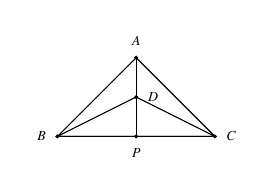
\begin{tikzpicture}
%[scale=0.5,>=stealth,point/.style={draw,circle,fill = green,inner sep=0.1pt},]
[scale=0.5,>=stealth, point/.style={draw,circle,fill = black,inner sep=0.1pt}]

% the coordinates of the vertices
\coordinate (A) at (2,2);
\coordinate (B) at (0,0);
\coordinate (C) at (4,0);
\coordinate (D) at (2,1);
\coordinate (P) at (2,0);


% the axis
\draw[thin,scale=0,-] (-1,0) -- (5.5,0);
\draw[thin,scale=0,-] (0,-2.5) -- (0,2.5);
\draw[thin,scale=0,-] (0,-2.5) -- (0,2.5);

% the edges of the triangle
\draw (B) -- (A) -- (C)-- cycle;
\draw (B) -- (D) -- (C)-- cycle;
\draw[-] (A) -- (D) ;
\draw[-] (P) -- (D) ;


% labelling the vertices
\node[point,label={above:\tiny $A$}] at (A) {};
\node[point,label={left:\tiny $B$}] at (B) {};
\node[point,label={right:\tiny $C$}] at (C) {};
\node[point,label={right:\tiny $D$}] at (D) {};
\node[point,label={below:\tiny $P$}] at (P) {};



%
\end{tikzpicture}
}
\caption{Iso-sceles Triangles by Latex-Tikz}
\label{fig:iso_scelen}	
\end{figure}

The above problem statement is depicted in the figure \ref{fig:iso_scelen} where the vertices are: $\vec{A} = \myvec{a_1\\a_2}$ , $\vec{B} = \myvec{0\\0}$, $\vec{C} = \myvec{c_1\\0}$, $\vec{D} = \myvec{d_1\\d_2}$ and $\vec{P} = \myvec{p_1\\0}$

From the problem statement we get that:
\begin{align}
\norm{\vec{A}-\vec{B}} = \norm{\vec{A}-\vec{C}}
\implies \norm{\vec{AB}} = \norm{\vec{AC}}
\end{align}
\label{cond1}

\begin{align}
\norm{\vec{D}-\vec{B}} = \norm{\vec{D}-\vec{C}}
\implies \norm{\vec{DB}} = \norm{\vec{DC}}
\end{align}
\label{cond2}

Now, let $\vec{P}$ = k$\vec{C}$ as $\vec{P}$ is on $\vec{BC}$.
So, 
\begin{align}
\myvec{p_1\\0} = k\myvec{c_1\\0}
\implies p_1 = kc_1
\end{align}

Now, squaring both side of the equation \ref{cond1},
\begin{align}
\norm{\vec{A}-\vec{B}}^2 = \norm{\vec{A}-\vec{C}}^2\\
\implies a_1^2 + a_2^2 = (a_1- c_1)^2 + a_2^2\\
\implies c_1^2 = 2a_1 c_1\\
\implies c_1(c_1 - 2a_1) = 0\label{cond3}
\end{align}
\label{cond3}
So, either $c_1$ = 0 or $c_1$ = 2$a_1$. As $c_1$ = 0 is not possible, so $c_1$ = 2$a_1$.

Similarly, squaring both side of the equation \ref{cond2},
\begin{align}
\norm{\vec{D}-\vec{B}}^2 = \norm{\vec{D}-\vec{C}}^2\\
\implies d_1^2 + d_2^2 = (d_1- c_1)^2 + d_2^2\\
\implies c_1^2 = 2d_1 c_1\\
\implies c_1(c_1 - 2d_1) = 0\label{cond4}
\end{align}
\label{cond4}

So, either $c_1$ = 0 or $c_1$ = 2$d_1$. As $c_1$ = 0 is not possible, so $c_1$ = 2$d_1$.

So, it is observed that $d_1$ = $a_1$.
So we can say that $\vec{A} = \myvec{a_1\\a_2}$ and $\vec{D} = \myvec{a_1\\d_2}$ and as $\vec{AD}$ is extended to intersect $\vec{BC}$ at $\vec{P}$, so $\vec{P} = \myvec{a_1\\0}$.

Now, $\norm{\vec{BP}}$ = $p_1$ = $a_1$ and $\norm{\vec{CP}}$ = $\sqrt{(2a_1 - a_1)^2}$= $a_1$.

For $\triangle DBC$ being iso-scelen, $\angle DBC$ = $\angle DCB$. 
\begin{align}
\angle DBC = \angle DCB\\
\implies \frac{\vec{CD}^T \vec{CP}}{\norm{\vec{CD}}\norm{\vec{CP}}}=\frac{\vec{BD}^T \vec{BP}}{\norm{\vec{BD}}\norm{\vec{BP}}}\\
\implies k\norm{\vec{CP}} = (1-k)\norm{\vec{BP}}\\
\implies k \times a_1 = (1-k) \times a-1 \\
\implies k= \frac{1}{2}
\end{align}

Now, let the angle between $\vec{AB}$ and $\vec{AP}$ is $\theta_1$ and the angle between $\vec{AP}$ and $\vec{AC}$ is $\theta_2$.
\begin{align}
\cos\theta_1 = \frac{\vec{AB}^T \vec{AP}}{\norm{\vec{AB}}\norm{\vec{AP}}}\\
\implies \cos\theta_1 = \frac{a_1^2 - ka_1c_1 + a_2^2}{\norm{\vec{AB}}\norm{\vec{AP}}}\\
\implies \cos\theta_1 = \frac{a_1^2 - 2ka_1^2 + a_2^2}{\norm{\vec{AC}}\norm{\vec{AP}}}
\end{align}

Now, putting the value of k = $\frac{1}{2}$,
\begin{align}
\cos\theta_1 = \frac{a_2^2}{\norm{\vec{AC}}\norm{\vec{AP}}}
\end{align}

Similarly,
\begin{align}
\cos\theta_2 = \frac{\vec{AC}^T \vec{AP}}{\norm{\vec{AC}}\norm{\vec{AP}}}\\
\implies \cos\theta_2 = \frac{-a_1^2 + 2ka_1^2 + a_2^2}{\norm{\vec{AC}}\norm{\vec{AP}}}
\end{align}

And now, putting the value of k = $\frac{1}{2}$,
\begin{align}
 \cos\theta_2 = \frac{a_2^2}{\norm{\vec{AC}}\norm{\vec{AP}}}
\end{align}

So, it can be easily observed that $\theta_1$ = $\theta_2$ (considering the principle value) and this proves that $\vec{AP}$ bisects $\angle A$.

Now, let consider the angle between $\vec{DP}$ and $\vec{BP}$ is $\phi$.
\begin{align}
\cos\phi = \frac{\vec{PD}^T \vec{PB}}{\norm{\vec{PD}}\norm{\vec{PB}}}\\
\implies \cos\phi = \frac{p_1(p_1 - d_1)}{\norm{\vec{PD}}\norm{\vec{PB}}}\\
\implies \cos\phi = \frac{p_1(2kd_1 - d_1)}{\norm{\vec{PD}}\norm{\vec{PB}}}\\
\implies \cos\phi = \frac{p_1(d_1 - d_1)}{\norm{\vec{PD}}\norm{\vec{PB}}}\\
\implies \cos\phi = 0\\
\implies \phi = 90 \degree
\end{align}

so, we can say that $\vec{DP}$ is perpendicular to $\vec{BC}$ and this indicates that $\vec{AP}$ is the perpendicular bisector of $\vec{BC}$.
%Hence, the above problem statement  is proved.
\renewcommand{\theequation}{\theenumi}
%\begin{enumerate}[label=\thesection.\arabic*.,ref=\thesection.\theenumi]
%\numberwithin{equation}{enumi}
%\item Verification of the above problem using python code.\\
%%\solution The  following Python code generates Fig. \ref{fig:point_distance}
%%\begin{lstlisting}
%%codes/det_check.py
%%\end{lstlisting}
%
%\end{enumerate}

\end{document}



